\documentclass{article}
\usepackage{amsmath}
\usepackage{cancel}
\usepackage{graphicx}

\allowdisplaybreaks
\begin{document}

\section*{Ejercicio 1.(2,5 ptos)}
Descomponer $F(s) = \dfrac{2s - 8}{s^2 - 5s + 6}$ en fracciones parciales y calcular $\mathcal{L}^{-1}[F(s)]$
\begin{align*}
    F(s) = 2\cdot\dfrac{s - 4}{s^2 - 5s + 6}\rightarrow \dfrac{s - 4}{s^2 - 5s + 6}
\end{align*}
Factorizamos el denominador:
\begin{align*}
    s &= \frac{-(-5) \pm \sqrt{(-5)^2 - 4\cdot1\cdot6}}{2\cdot1}
    = \frac{5 \pm \sqrt{25 - 24}}{2}
    = \frac{5 \pm 1}{2} \\
\end{align*}
Las raíces son:
\begin{align*}
    \rightarrow s_1 &= \frac{5 + 1}{2} = \frac{6}{2} = 3 \\
    \rightarrow s_2 &= \frac{5 - 1}{2} = \frac{4}{2} = 2
\end{align*}
La descomposición en fracciones simples se define según la expresión:
\begin{align*}
    \dfrac{s - 4}{(s - 3) (s - 2)} = \dfrac{A_1}{s - 3} + \dfrac{A_2}{s - 2}
\end{align*}
Calculamos los coeficientes $A_i$:
\begin{align*}
    \rightarrow A_1 
    &= \lim_{s \to 3} \dfrac{\cancel{(s - 3)} (s - 4)}{\cancel{(s - 3)}(s - 2)}
    = \lim_{s \to 3} \dfrac{s - 4}{s - 2}
    = \dfrac{3 - 4}{3 - 2}
    = \dfrac{-1}{1}
    = -1 \\
    \rightarrow A_2 
    &= \lim_{s \to 2} \dfrac{\cancel{(s - 2)} (s - 4)}{(s - 3) \cancel{(s - 2)}}
    = \lim_{s \to 2} \dfrac{s - 4}{s - 3}
    = \dfrac{2 - 4}{2 - 3}
    = \dfrac{-2}{-1}
    = 2
\end{align*}
Obtenemos la expresión de $F(s)$ como suma de fracciones:
\begin{align*}
    F(s) 
    = 2\cdot\left(\dfrac{-1}{s - 3} + \dfrac{2}{s - 2}\right)
    = \dfrac{-2}{s - 3} + \dfrac{4}{s - 2} 
\end{align*}
Aplicamos la transformada inversa $\mathcal{L}^{-1}$,
que por linealidad se puede expresar como:
\begin{align*}
    \mathcal{L}^{-1}[F(s)]
    = (-2)\cdot\mathcal{L}^{-1}\left[\dfrac{1}{s - 3}\right]
    + 4\cdot\mathcal{L}^{-1}\left[\dfrac{1}{s - 2}\right]
\end{align*}
A partir de Table of Laplace Transforms 7 llegamos al resultado buscado:
\begin{align*}
    \mathcal{L}^{-1}[F(s)]
    = (-2) \cdot e^{3t} + 4 \cdot e^{2t}
\end{align*}

\section*{Ejercio 2.(2,5 ptos)}
Descomponer $F(s) = \dfrac{8s^2 - 7s + 6}{s^2 (s - 2)}$ en fracciones parciales y calcular $\mathcal{L}^{-1}[F(s)]$
Las raíces del denominador son:
\begin{align*}
    \rightarrow s_1 &= 0 \quad \text{(doble)} \\
    \rightarrow s_2 &= 2 \quad \text{(simple)}
\end{align*}
La descomposición en fracciones simples se define según la expresión:
\begin{align*}
    \dfrac{8s^2 - 7s + 6}{s^2 (s - 2)}
    = \dfrac{A_1}{s}
    + \dfrac{A_2}{s^2}
    + \dfrac{B_1}{s - 2}
\end{align*}
Calculamos los coeficientes $A_i$ utilizando la expresión general para raíces reales múltiples:
\begin{align*}
    A_k
    = \dfrac{1}{(m - k)!} \lim_{s \to p} \left[\dfrac{d^{m-k}}{ds^{m-k}}\left((s - p)^m \dfrac{N(s)}{D(s)}\right)\right]
\end{align*}
\begin{enumerate}
    \item p es la raíz del denominador relacionada con los coeficientes $A_i$
    \item k es el índice del coeficiente que estamos calculando ($A_k$)
    \item m es la multiplicidad de la raíz
\end{enumerate}
Para $A_2$ se simplifica la expresión al ser 
m=2 y k=2 ($m-k = 0$)
\begin{align*}
    A_2 
    &= \lim_{s \to 0} \dfrac{\cancel{s^2} (8s^2 - 7s + 6)}{\cancel{s^2}(s - 2)}
    = \lim_{s \to 0} \dfrac{8s^2 - 7s + 6}{s - 2} 
    = \dfrac{8 \cdot 0^2 - 7 \cdot 0 + 6}{0 - 2} 
    = \dfrac{6}{-2}
    = -3\\ 
    A_2 &= -3 \\
\end{align*}
Calculamos $A_1$ utilizando la expresión general con m=2 y k=1 ($m-k = 1$)
\begin{align*}    
    A_1
    &= \dfrac{1}{1!}\lim_{s \to 0} \left[\dfrac{d}{ds}\left((s-0)^2\dfrac{8s^2 - 7s + 6}{s^2 (s - 2)}\right)\right]
    = \lim_{s \to 0} \left[\dfrac{d}{ds}\left(\cancel{s^2}\dfrac{8s^2 - 7s + 6}{\cancel{s^2} (s - 2)}\right)\right] = \\
    &= \lim_{s \to 0} \dfrac{(16s - 7)(s - 2) - (8s^2 - 7s + 6) \cdot 1}{(s - 2)^2} = \\ 
    &= \dfrac{(16 \cdot 0 - 7)(0 - 2) - (8 \cdot 0^2 - 7 \cdot 0 + 6)}{(0 - 2)^2} 
    = \dfrac{14 - 6}{4}
    = \dfrac{8}{4}
    = 2 \\
    A_1 &= 2
\end{align*}
Calculamos $B_1$ de manera análoga a $A_2$
\begin{align*}
    B_1
    &= \lim_{s \to 2} \dfrac{\cancel{(s - 2)} (8s^2 - 7s + 6)}{s^2 \cancel{(s - 2)}}
    = \lim_{s \to 2} \dfrac{8s^2 - 7s + 6}{s^2} 
    = \dfrac{8 \cdot 2^{\cancel{2}} - 7 \cdot \cancel{2} + \cancelto{3}{6}}{2^{\cancel{2}}} = \\
    &= \dfrac{16 - 7 + 3}{2}
    = \dfrac{12}{2}
    = 6
\end{align*}
Podemos expresar $F(s)$ como suma de fracciones:
\begin{align*}
    F(s)
    = \dfrac{2}{s}
    + \dfrac{-3}{s^2}
    + \dfrac{6}{s - 2}
\end{align*}
Aplicamos la transformada inversa $\mathcal{L}^{-1}$,
que por linealidad se puede expresar como:
\begin{align*}
    \mathcal{L}^{-1}[F(s)]
    = 2\cdot\mathcal{L}^{-1}\left[\dfrac{1}{s}\right]
    + (-3)\cdot\mathcal{L}^{-1}\left[\dfrac{1}{s^2}\right]
    + 6\cdot\mathcal{L}^{-1}\left[\dfrac{1}{s - 2}\right]
\end{align*}
A partir de Table of Laplace Transforms 1, 2 y 7  llegamos al resultado buscado:
\begin{align*}
    \mathcal{L}^{-1}[F(s)]
    = 2 \cdot 1
    + (-3) \cdot t
    + 6 e^{2t}
    = 2
    - 3t
    + 6 e^{2t}
\end{align*}
\section*{Ejercicio 3. (3,5 ptos)}
Obtenga las transformadas inversas $g(t)$ de las siguientes funciones $G(s)$
\begin{align*}
    G(s) 
    &= \dfrac{4}{s + 6}
    = 4 \cdot \dfrac{1}{s - (-6)} \\
    \rightarrow\mathcal{L}^{-1}[G(s)]&
    = 4 \cdot e^{-6t} \\
    \\ \hline \\
    G(s) 
    &= \dfrac{2}{s^4}
    = 2 \cdot \dfrac{1}{s^4} \\
    \rightarrow\mathcal{L}^{-1}[G(s)]&
    = 2 \cdot \dfrac{t^{4-1}}{(4-1)!}
    = 2 \cdot \dfrac{t^{3}}{3!}
    = \dfrac{t^3}{3} \\    
    \\ \hline \\
    G(s) 
    &= \dfrac{2s}{s^2 + 3}
    = 2 \cdot \dfrac{s}{s^2 + (\sqrt{3})^2} \\
    \rightarrow\mathcal{L}^{-1}[G(s)]&
    = 2 \cos(\sqrt{3}t) \\
    \\ \hline \\
    G(s) 
    &= \dfrac{3}{s^2 + 16}
    = 3 \cdot \dfrac{1}{s^2 + 4^2} \\
    \rightarrow\mathcal{L}^{-1}[G(s)]&
    = \dfrac{3}{4} \sin(4t) \\
    \\ \hline \\
    G(s) 
    &= \dfrac{2s + 4}{s^3} + \dfrac{3s - 14}{s^2 + 9} = \\
    &= 2 \cdot \left(\dfrac{\cancel{s}}{\cancel{s} \cdot s^2} + 2 \cdot \dfrac{1}{s^3}\right) 
    + 3 \cdot \dfrac{s}{s^2 + 3^2}
    - 14 \cdot \dfrac{1}{s^2 + 3^2} \\
    \rightarrow\mathcal{L}^{-1}[G(s)]&
    = 2 \left(t + \cancel{2} \cdot \dfrac{t^2}{\cancel{2!}}\right)
    + 3 \cos(3t)
    - \dfrac{14}{3} \sin(3t) = \\
    &= 2t + 2t^2 + 3\cos(3t) - \dfrac{14}{3} \sin(3t) \\    
    \\ \hline \\
    G(s) 
    &= \dfrac{8}{2s - 3} 
    + \dfrac{6s - 10}{16s^2 + 9} = \\
    &= 8 \cdot \dfrac{\dfrac{1}{2}}{\dfrac{\cancel{2}s}{\cancel{2}} - \dfrac{3}{2}}
    + 6 \cdot \dfrac{\dfrac{s}{16}}{\dfrac{\cancel{16}s^2}{\cancel{16}} + \dfrac{9}{16}} 
    -10 \cdot \dfrac{\dfrac{1}{16}}{\dfrac{\cancel{16}s^2}{\cancel{16}} + \dfrac{9}{16}} = \\
    &= 4 \cdot \dfrac{1}{s - \dfrac{3}{2}}
    + \dfrac{3}{8} \cdot \dfrac{s}{s^2 + \left(\dfrac{3}{4}\right)^2} 
    - \dfrac{5}{8} \cdot \dfrac{1}{s^2 + \left(\dfrac{3}{4}\right)^2} \\
    \rightarrow\mathcal{L}^{-1}[G(s)]&
    = 4 \cdot e^{\frac{3}{2}}
    + \dfrac{3}{8} \cos\left(\dfrac{3}{4}t\right)
    - \dfrac{5}{8} \cdot \dfrac{1}{\dfrac{3}{4}}\sin\left(\dfrac{3}{4}t\right) = \\
    &= 4 \cdot e^{\frac{3}{2}}
    + \dfrac{1}{2} \cos\left(\dfrac{3}{4}t\right)
    - \dfrac{5}{6} \sin\left(\dfrac{3}{4}t\right)
\end{align*}
\section*{Ejercicio 4. (1,5 ptos)}
Para el sistema masa-resorte-amortiguador de la figura, obtenga la función de transferencia \(G(s)\) (nombre dado a la función racional que representa a un sistema compuesto por polos y ceros y es el cociente de la salida sobre la entrada en el dominio de Laplace), donde se supone cero en todas las condiciones iniciales. Además, obtenga una expresión del desplazamiento \(X(s)\) de la masa \(m\), cuando le aplica una entrada a manera de fuerza \(f(t)\) \\
\begin{figure}[h]
    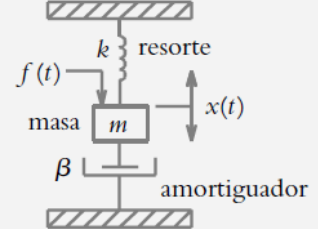
\includegraphics[scale=0.5]{masa-muelle-resorte.png}
    \centering
\end{figure}
\pagebreak
\\
Como consideración inicial elegimos los ejes del sistema, en este caso solo nos interesa el eje vertical (en adelante eje x) tomamos como \(x=0\) la posición de equilibrio, con sentido vertical hacia arriba, es decir, hacia valores positivos de \(x\) los vectores posición, velocidad y aceleración serán positivos (el signo de las fuerzas se obtiene del signo de la aceleración que aplican \(F = m \cdot a\))
\begin{figure}[h]
    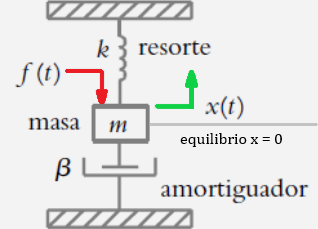
\includegraphics[scale=0.5]{masa-muelle-resorte-ejes.png}
    \centering
\end{figure}
\\
Fuerzas que intervienen:
\begin{itemize}
    \item Fuerza del muelle
    \subitem \(F_k = k \cdot \Delta L = k \cdot (L-L_0)\) \\
    \(L_0\) es la enlongación del muelle en la posición de equilibrio, para nuestro sistema de coordenadas \(L = x\) y \(L_0 = 0\) y por tanto la fuerza del muelle queda \(F_k = k \cdot x(t)\). Si la posición de la masa (\(x(t)\)) se encuentra por encima de la posición de equilibrio será una fuerza negativa (y positiva en caso contrario).

    \item Fuerza del amortiguador
    \subitem \(F_\beta = \beta \cdot x'(t)\) \\
    Si la velocidad de la masa (\(x'(t)\)) es en sentido de las \(x\) positivas será una fuerza negativa (y positiva en caso contrario).

    \item Fuerza de entrada
    \subitem \(f(t)\) \\
    Siguiendo nuestro sistema de coordenadas, es negativa al ir en sentido contrario de las \(x\) positivas.

    \item[Nota:] Por simplicidad y al no especificarse en el enunciado ignoraremos la presencia de un posible campo gravitatorio (Y así poder reproducir el ejemplo de los apuntes). 
\end{itemize}
Ecuación del modelo:
\begin{align*}
    \sum F 
    = 
    m \cdot a
    = F_k + F_\beta + u(t) \\
    m \cdot x''(t)
    = 
    - k \cdot x(t)
    - \beta \cdot x'(t)
    - f(t)
\end{align*}
Reordenando términos queda:
\begin{align*}
    m \cdot x''(t)
    + \beta \cdot x'(t)
    + k \cdot x(t) 
    = - f(t)
\end{align*}
Aplicamos la transformada de Laplace a ambos lados para pasar al dominio \(s\). 
\begin{align*}
    m \cdot s^2 \cdot X(s)
    + \beta \cdot s \cdot X(s)
    + k \cdot X(s)
    = 
    F(s)
\end{align*}
\begin{align*}
    \dfrac{X(s)}{F(s)}
    =
    \dfrac{1}{m \cdot s^2 + \beta \cdot s + k}
    =
    \dfrac{\dfrac{1}{m}}{s^2 + \dfrac{c}{m} \cdot s + \dfrac{k}{m}}
\end{align*}
La forma canónica para sistemas de segundo orden:
\begin{align*}
    \dfrac{X(s)}{F(s)}
    =
    K \cdot \dfrac{w_n^2}{s^2 + 2 \cdot \xi \cdot w_n \cdot s + w_n^2}
\end{align*}
Identificando términos con nuestro sistema:

\end{document}
